 \section{درونیابی لاگرانژ و اسپلاین مکعبی}
 در این بخش، هدف یافتن توابع درونیاب برای نقاط داده‌شده در صورت پروژه است. نقاط مشخص‌شده عبارتند از:
 $ (1,1) $، $ (2,3) $، $ (3,5) $، $ (4,8) $، $ (5,5) $ و $ (6,2) $.
 برای این داده‌ها، دو روش درونیابی لاگرانژ\footnote{\lr{Lagrange Interpolation}} و اسپلاین مکعبی طبیعی\footnote{\lr{Natural Cubic Spline}} در محیط پایتون\footnote{\lr{Python}} پیاده‌سازی شده است.
 
 \subsection{مراحل و نحوه پیاده‌سازی الگوریتم‌ها}
 پروژه پایتون مربوط به این بخش شامل گام‌های زیر است:
 \begin{enumerate}
  \item \textbf{تعریف و مقداردهی اولیه نقاط:} ابتدا نقاط به‌صورت دو آرایه مجزا برای مولفه‌های $ x $ و $ y $ در کتابخانه نام‌پای\footnote{\lr{NumPy}} تعریف می‌شوند.
  \item \textbf{درونیابی لاگرانژ:} برای درونیابی لاگرانژ و جلوگیری از ناپایداری‌های عددی معمول، از کلاس پیشرفته \lstinline|BarycentricInterpolator| در کتابخانه سای‌پای\footnote{\lr{SciPy}} استفاده شده است.
  \item \textbf{استخراج محاسباتی ضابطه ریاضی:} به دلیل اینکه کتابخانه‌های محاسبات عددی صرفاً خروجی عددی می‌دهند، با استفاده از کتابخانه سیم‌پای\footnote{\lr{SymPy}} فرمول نمادین پایه‌های لاگرانژ پیاده‌سازی و در نهایت با دستور \lstinline|expand| ساده‌سازی شده است تا ضابطه دقیق باز شود.
  \item \textbf{درونیابی اسپلاین مکعبی:} با استفاده از کلاس \lstinline|CubicSpline| و با تنظیم پارامتر \lstinline|bc_type='natural'| شرط مرزی صفر بودن مشتق دوم در نقاط ابتدایی و انتهایی اعمال شده و ضرایب توابع تکه‌ای استخراج گردیده‌اند.
  \item \textbf{تصویرسازی و ذخیره‌سازی:} با کمک کتابخانه مت‌پلات‌لیب\footnote{\lr{Matplotlib}} هر دو نمودار به همراه نقاط اصلی رسم و با کیفیت بالا ذخیره می‌شوند.
 \end{enumerate}
 
 \subsection{کد پایتون پیاده‌سازی شده}
 کد کامل پایتون که برای انجام محاسبات این بخش نوشته شده، به شرح زیر است:
 
 \begin{latin}
  \begin{lstlisting}
   import numpy as np
   import matplotlib.pyplot as plt
   from scipy.interpolate import BarycentricInterpolator, CubicSpline
   from sympy import symbols, expand
   
   # 1. Define the data points given in the project prompt
   x_data = np.array([1, 2, 3, 4, 5, 6])
   y_data = np.array([1, 3, 5, 8, 5, 2])
   
   print("--- Part 1: Lagrange Interpolation ---")
   # 2. Perform Lagrange interpolation using BarycentricInterpolator
   lagrange_interpolator = BarycentricInterpolator(x_data, y_data)
   
   # Extract the exact mathematical formula using sympy for clear display
   x_sym = symbols('x')
   lagrange_expr = 0
   for i in range(len(x_data)):
       # Construct Lagrange basis polynomials
       p = 1
       for j in range(len(x_data)):
           if i != j:
               p *= (x_sym - x_data[j]) / (x_data[i] - x_data[j])
       lagrange_expr += y_data[i] * p
   
   lagrange_simplified = expand(lagrange_expr)
   print("Exact formula for Lagrange interpolating polynomial:")
   print(f"L(x) = {lagrange_simplified}\n")
   
   print("--- Part 2: Spline Interpolation ---")
   # 3. Perform Cubic Spline interpolation (Natural type)
   cs = CubicSpline(x_data, y_data, bc_type='natural')
   
   print("Exact piecewise formulas for the Cubic Spline (per interval):")
   for i in range(len(x_data) - 1):
       coeffs = cs.c[:, i]
       d, c, b, a = coeffs[0], coeffs[1], coeffs[2], coeffs[3]
       print(f"Interval [{x_data[i]}, {x_data[i+1]}]:")
       print(f"  S_{i}(x) = {a} + {b:.4f}(x - {x_data[i]}) + {c:.4f}(x - {x_data[i]})^2 + {d:.4f}(x - {x_data[i]})^3")
			
   # 4. Plotting the results for the final report
   x_plot = np.linspace(1, 6, 500)
   y_lagrange_plot = lagrange_interpolator(x_plot)
   y_spline_plot = cs(x_plot)
			
   plt.figure(figsize=(10, 6))
   plt.scatter(x_data, y_data, color='red', zorder=5, label='Original Data Points')
   plt.plot(x_plot, y_lagrange_plot, label='Lagrange Interpolation', linestyle='--', color='blue')
   plt.plot(x_plot, y_spline_plot, label='Natural Cubic Spline', linestyle='-', color='green')
   plt.title('Comparison of Lagrange and Cubic Spline Interpolation')
   plt.xlabel('X')
   plt.ylabel('Y')
   plt.grid(True, linestyle=':', alpha=0.6)
   plt.legend()
   plt.savefig('interpolation_plot.png', dpi=300)
  \end{lstlisting}
 \end{latin}
	
 \subsection{خروجی دقیق برنامه در محیط ترمینال}
 پس از اجرای کد فوق، خروجی‌های دقیق ریاضی به صورت متنی در ترمینال به شرح زیر نمایش داده می‌شوند:
	
 \begin{latin}
  \begin{verbatim}
   --- Part 1: Lagrange Interpolation ---
   Exact formula for Lagrange interpolating polynomial:
   L(x) = 7*x**5/40 - 71*x**4/24 + 147*x**3/8 - 1249*x**2/24 + 1369*x/20 - 31
			
   --- Part 2: Spline Interpolation ---
   Exact piecewise formulas for the Cubic Spline (per interval):
   Interval [1, 2]:
     S_0(x) = 1.0 + 2.1866(x - 1) + 0.0000(x - 1)^2 + -0.1866(x - 1)^3
   Interval [2, 3]:
     S_1(x) = 3.0 + 1.6268(x - 2) + -0.5598(x - 2)^2 + 0.9330(x - 2)^3
   Interval [3, 4]:
     S_2(x) = 5.0 + 3.3062(x - 3) + 2.2392(x - 3)^2 + -2.5455(x - 3)^3
   Interval [4, 5]:
     S_3(x) = 8.0 + 0.1483(x - 4) + -5.3971(x - 4)^2 + 2.2488(x - 4)^3
   Interval [5, 6]:
     S_4(x) = 5.0 + -3.8995(x - 5) + 1.3493(x - 5)^2 + -0.4498(x - 5)^3
  \end{verbatim}
 \end{latin}
	
 \subsection{ضابطه چندجمله‌ای درونیاب لاگرانژ}
 با توجه به خروجی سیستم، ضابطه دقیق ریاضی ساده‌شده‌ی چندجمله‌ای لاگرانژ به صورت زیر است:
 \[
 L(x) = \frac{7}{40}x^5 - \frac{71}{24}x^4 + \frac{147}{8}x^3 - \frac{1249}{24}x^2 + \frac{1369}{20}x - 31.
 \]
	
 \subsection{ضابطه تکه‌ای درونیاب اسپلاین مکعبی}
 فرمول ریاضی تکه‌ای توابع درجه سوم برازش‌شده بر روی فواصل مجاور به شرح زیر است:
 \begin{align*}
  S_0(x) &= 1.0 + 2.1866(x - 1) - 0.1866(x - 1)^3, \quad & x \in [1, 2], \\
  S_1(x) &= 3.0 + 1.6268(x - 2) - 0.5598(x - 2)^2 + 0.9330(x - 2)^3, \quad & x \in [2, 3], \\
  S_2(x) &= 5.0 + 3.3062(x - 3) + 2.2392(x - 3)^2 - 2.5455(x - 3)^3, \quad & x \in [3, 4], \\
  S_3(x) &= 8.0 + 0.1483(x - 4) - 5.3971(x - 4)^2 + 2.2488(x - 4)^3, \quad & x \in [4, 5], \\
  S_4(x) &= 5.0 - 3.8995(x - 5) + 1.3493(x - 5)^2 - 0.4498(x - 5)^3, \quad & x \in [5, 6].
 \end{align*}
	
 \subsection{نمودار مقایسه‌ای و تحلیل کامل رفتار توابع}
 شکل~\ref{fig:interpolation} نشان‌دهنده نمودار خروجی حاصل از اجرای کد پایتون است.
	
 \begin{figure}[htbp]
  \centering
  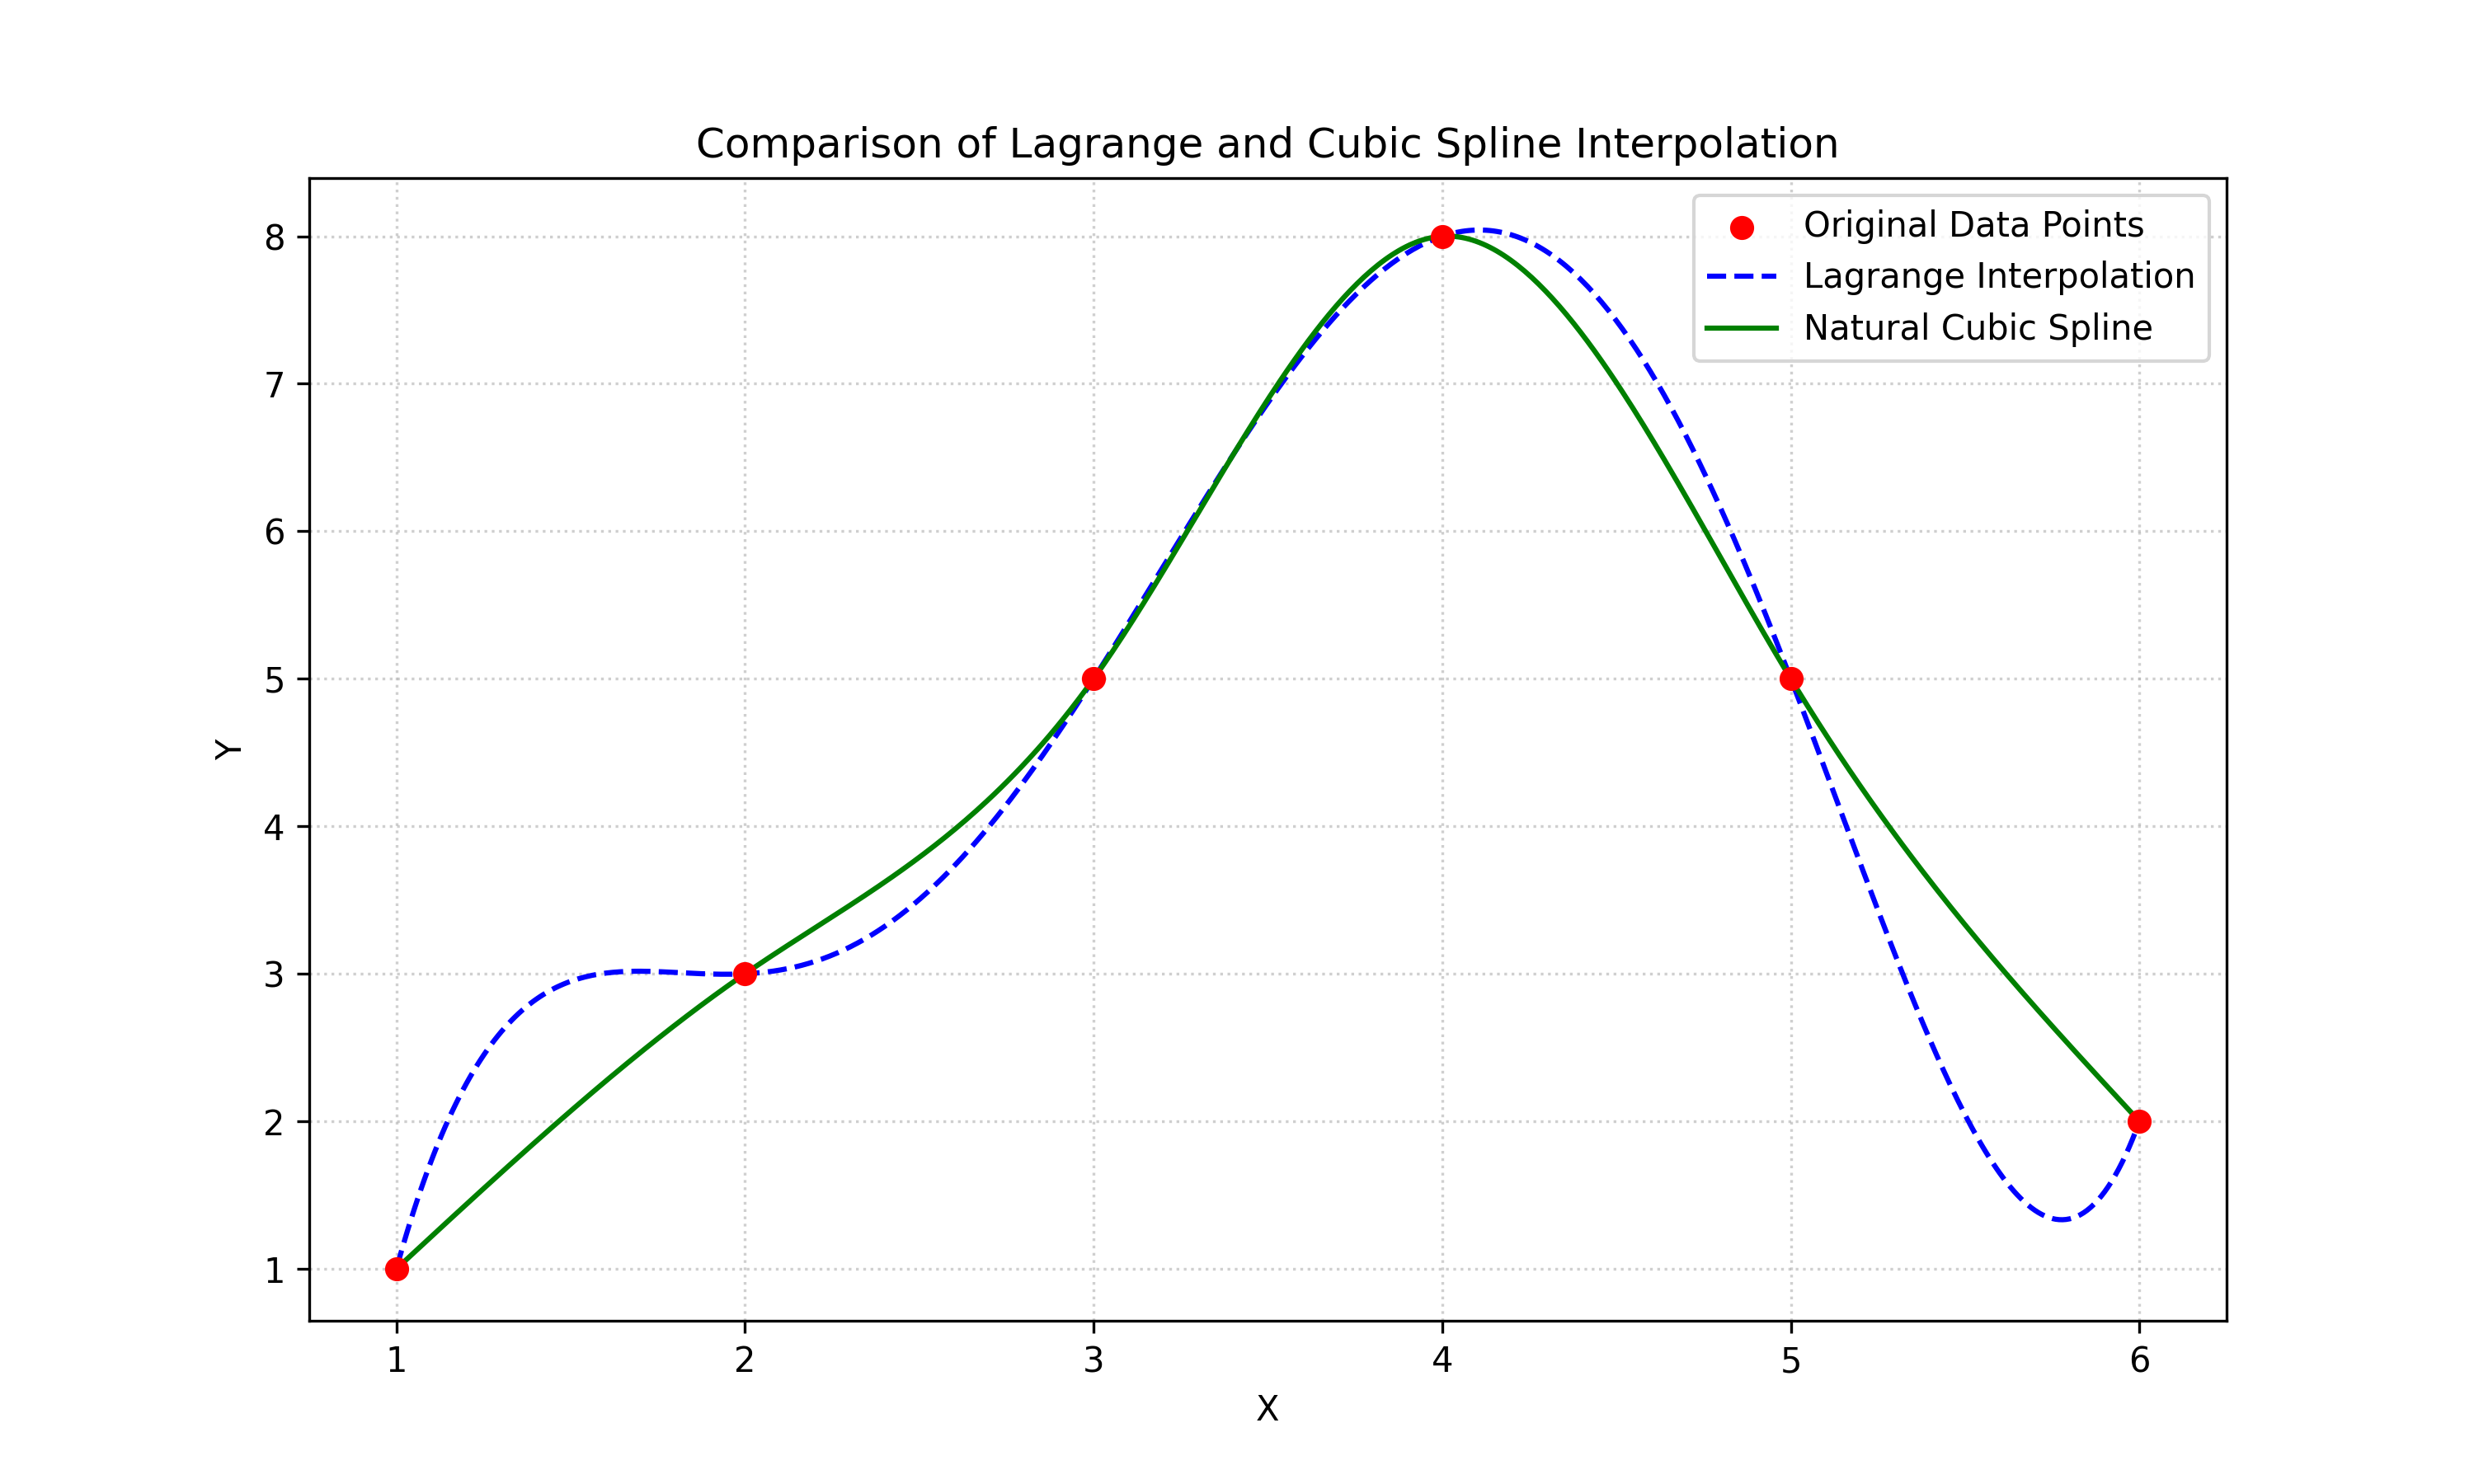
\includegraphics[width=0.85\textwidth]{interpolation_plot.png}
  \caption{نمودار مقایسه عملکرد درونیابی لاگرانژ و اسپلاین مکعبی طبیعی بر روی نقاط داده‌شده.}
  \label{fig:interpolation}
 \end{figure}
	
 تحلیل ریاضی رفتار این دو منحنی نشان می‌دهد که هر دو روش با موفقیت کامل از تمامی ۶ نقطه داده‌شده عبور کرده‌اند؛ اما تفاوت رفتار نوسانی عظیمی با یکدیگر دارند. چندجمله‌ای لاگرانژ به دلیل برخورداری از درجه بالا ($ n - 1 = 5 $)، در بازه‌های ابتدایی و انتهایی دچار نوسانات شدید خارج از محدوده داده‌ها شده است. این رفتار نوسانی نامطلوب به پدیده رانگ\footnote{\lr{Runge's phenomenon}} معروف است که نشان می‌دهد توابع چندجمله‌ای درجه بالا برای نقاط با فواصل مساوی گزینه‌ی مناسبی نیستند.
	
 در مقابل، روش اسپلاین مکعبی به دلیل ماهیت تکه‌ای بودن، در هر بازه تنها از توابع درجه ۳ استفاده می‌کند. برقراری شروط پیوستگی هم‌زمانِ تابع، مشتق اول و مشتق دوم در نقاط گره‌ای در کنار شرط مرزی طبیعی (صفر بودن مشتق دوم در پایانه‌ها)، سبب شده است تا منحنی اسپلاین رفتاری بسیار پایدار، نرم، عاری از هرگونه نوسان کاذب و کاملاً منطبق بر روند توزیع داده‌ها ارائه دهد.
